% Indicate the main file. Must go at the beginning of the file.
% !TEX root = ../main.tex

%----------------------------------------------------------------------------------------
% CHAPTER TEMPLATE
%----------------------------------------------------------------------------------------


\chapter{Resultate} % Main chapter title

\label{Chapter4} % Change X to a consecutive number; for referencing this chapter elsewhere, use \ref{ChapterX}

%----------------------------------------------------------------------------------------
% SECTION 1
%----------------------------------------------------------------------------------------
In diesem Kapitel erfolgt eine Erläuterung der Resultate, die durch die Durchführung der oben beschriebenen Methoden erzielt werden. Dafür stehen, wie bereits im Kapitel \secref{sec:Datengrundlagen} erwähnt, 71 Repositories zur Verfügung. 

Des Weiteren sollen die folgenden Hypothesen anhand von Projekten der Studierenden untersucht werden.

\hypothese{hypothese1}{
Gegen Ende des Projekts werden Pull Requests schneller gemergt.
}

Die Projekte haben ein festes Ziel und einen festen Abgabetermin. Aus eigener Erfahrung der Autoren schieben Studierende gerne Arbeiten vor sich her und generieren dadurch mehr Arbeit für das Ende des Projektes. Aus diesem Grund gehen wir davon aus, dass Pull Requests gegen Ende des Projekts schneller bearbeitet werden.

\hypothese{hypothese2}{
Teilzeitstudierende nutzen Pull Requests effizienter als Vollzeitstudierende.

}


Wir gehen davon aus, dass Teilzeitstudierende durch ihre Arbeit mehr Erfahrung in der Durchführung von Softwareprojekten und somit auch in der Verwendung von Pull Requests haben. Dies kann sich in Anzahl, Grösse aber auch Kommentare unterscheiden. 


Für die ersten Experimente wurden die Repositories der Racetrack-Projekte ausgewertet. Wie im Kapitel \secref{sec:Projektmodule} erwähnt, findet dieses Projekt im Kontext des Projektmoduls 2 als erstes Projekt statt. Dieses dauert ungefähr vier Wochen, wobei die genaue Anzahl der Tage pro Klasse variieren kann. Das Grundgerüst des Sourcecodes wird in der Aufgabenstellung mitgeliefert, was die Vergleichbarkeit der Projekte erhöht. Ausserdem haben die Studenten schon Erfahrung mit der Handhabung von PullRequests. 

\newpage
\section{Churn vs Latency}
Zur Klärung der \fref{forschungsfrage1}: "\textit{Besteht ein Zusammenhang zwischen der Latency eines Pull
Requests (Zeit bis zum Merge oder Schliessung) und dem Churn (Anzahl geänderter Codezeilen) des jeweiligen Pull Requests?}" werden die geminten Repository Daten in einem Jupiter Notebook aufbereitet und graphisch dargestellt. Dazu werden die im Kapitel \secref{sec:Metriken} erwähnten Metriken \textit{createTime} und \textit{closeTime} gemined und damit die einzelnen Latencies berechnet. Um die Latency-Daten besser vergleichen zu können, werden diese noch vom Datumsformat in Stunden umgerechnet. Des Weiteren werden die Metriken  \textit{additions} und  \textit{deleteions} aus den Pull Requests extrahiert, um den Churn zu berechnen.

\subsection{Datenanalyse}
Zum besseren Verständnis der \textit{latency}- und \textit{churn}- Werte wird zunächst eine allgemeine Analyse der Daten durchgeführt.
Die Analyse basiert auf 2435 extrahierten Pull Requests. Wovon im Durchschnitt 34.3 Pull Requests pro Repository erstellt werden. In der folgenden Tabelle werden die wichtigsten Kennzahlen aufgezeigt.


\begin{table}[htbp]
    \centering
    \caption{Kennzahlen zu \textit{Latency} und \textit{Churn}}
    \begin{tabular}{@{}lrr@{}}
        \toprule
        \textbf & \textbf{Latency (in Stunden)} & \textbf{Churn} \\
         \midrule
        Mittelwert & 18.6 & 278.2 \\
        Standardabweichung &  42.0  & 815.8 \\
        Minimum & 0.0008 & 0.0 \\
        1. Quartil (Q1) & 0.05 & 28.0 \\
        Median & 0.6 & 94.0 \\
        3. Quartil (Q3) &  16.4   & 251.0 \\
        Maximum & 416.3 & 17299.0 \\
        \bottomrule
    \end{tabular}
    \label{tab:deskriptive-kennzahlen}
\end{table}

Die Analyse zeigt, dass ein durchschnittlicher Pull Request eine Bearbeitungszeit von 18.6 Stunden hat, während der Median bei 0.6 Stunden liegt. Dies deutet darauf hin, dass die meisten Pull-Requests sehr schnell bearbeitet werden und nur wenige eine sehr lange Bearbeitungszeit haben. Das wird auch durch die Standardabweichung von 42 Stunden deutlich.

Ein ähnliches Bild zeigt sich beim Churn. Auch hier liegt der Mittelwert mit 278 Codezeilenänderungen höher und der Median bei nur 94 Änderungen. Die Standardabweichung zeigt ebenfalls eine grosse Streuung der Daten.

Diese Werte sind zusätzlich in den Boxplots in den Abbildungen \autoref{fig:boxplot-latency} und \autoref{fig:boxplot-churn} ersichtlich. 
In beiden Abbildungen ist der Box-Bereich auf der linken Seite kompakt und nahe bei Null. 
Die \autoref{fig:boxplot-latency} zeigt ebenfalls, dass viele Pull Requests schnell abgearbeitet werden, während wenige längere Bearbeitungszeiten aufweisen. Es zeigt ausserdem auf, dass es eine Reihe von Ausreissern gibt. Diese belaufen sich auf 14\,\% aller \textit{latencies}.

\begin{figure}[htbp]
    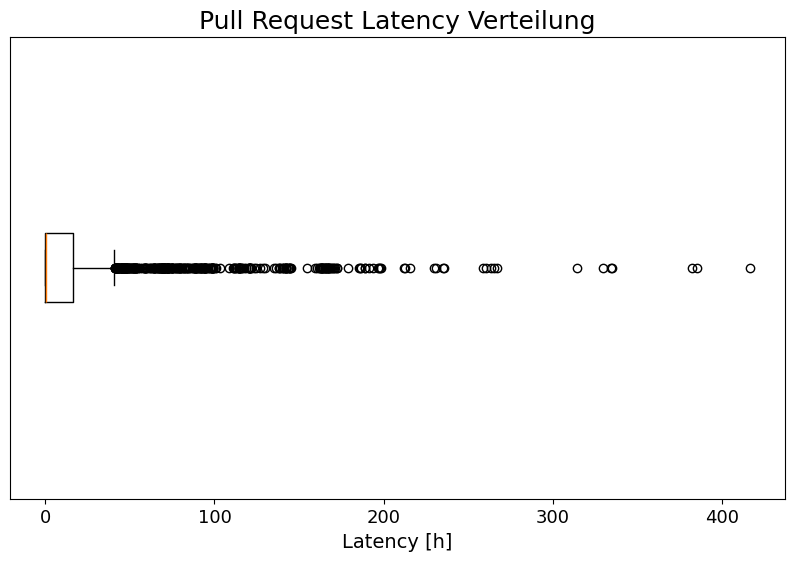
\includegraphics[width=0.8\textwidth]{Figures/boxplot-latency.png}
    \centering
    \caption{Boxplot Latency}
    \label{fig:boxplot-latency}
\end{figure}
 \newpage
Der Boxplot in der \autoref{fig:boxplot-churn} zeigt, dass es viele kleine Pull Requests mit wenigen Codezeilenänderungen gibt. Wie bereits bei der \textit{latency} wurde festgestellt, dass es eine Reihe von Ausreissern gibt, von denen einige besonders hervorstechen. Diese befinden sich bei über 10'000 Zeilenänderungen. In diesem Fall liegt die Anzahl der Ausreisser bei 9.6\,\%.

\begin{figure}[htbp]
    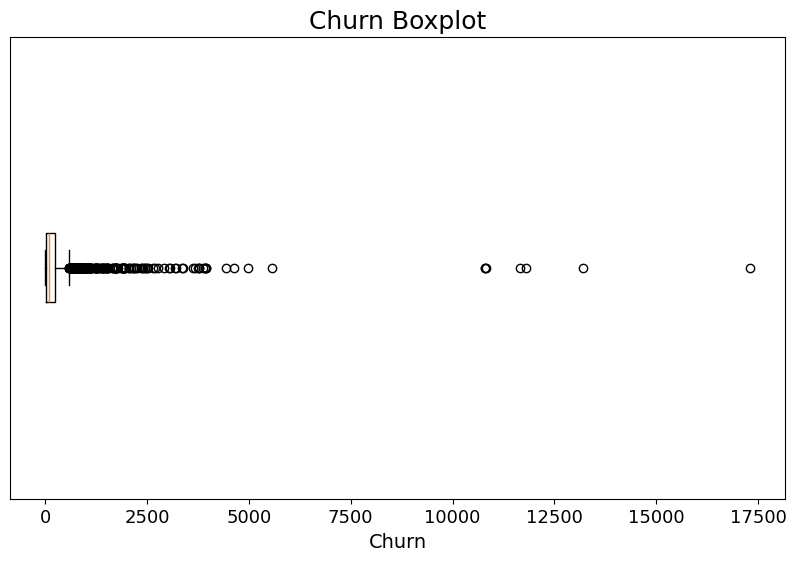
\includegraphics[width=0.8\textwidth]{Figures/boxplot-churn.png}
      \centering
    \caption{Boxplot Churn}
    \label{fig:boxplot-churn}
\end{figure}
\newpage
Werden die Ausreisser beider Metriken kumulativ aus allen Datensätzen herausgefiltert, bleiben 1887 Pull Requests übrig, was 77.5\,\% entspricht. Das Herausfiltern dieser Daten stellt einen erheblichen Eingriff in die Datenbasis dar und wird daher nicht pauschal vorgenommen.

\subsection{Ergebnisse}
Um festzustellen, ob zwischen den Metriken \textit{latency} und \textit{churn} ein Zusammenhang besteht wird die Spearman Rangkorrelation angewendet. Dafür wird die oben erwähnte \autoref{eqn:spearman} verwendet. Diese wird anhand der Phython Library \textit{pandas} berechnet. Als Ergebnis erreichte der Rangkorrelationskoeffizient einen Wert von 0.17. Dieser Wert liegt sehr Nahe bei null und zeigt somit keinen spezifischen Zusammenhang zwischen den beiden Metriken auf. 

Wie bereits erwähnt, weisen die Daten einen hohen Anteil an Ausreissern auf. Deshalb soll überprüft werden, ob die Metriken eine Korrelation besitzen, wenn diese Ausreisser herausgefiltert werden. In diesem Fall erhöht sich der Koeffizient auf 0.2, zeigt aber weiterhin keinen eindeutigen Zusammenhang zwischen den Metriken.

\textbf{Zusammenfassend kann zur \fref{forschungsfrage1} festgestellt werden, dass die Metriken \textit{latency} und \textit{churn} keinen Zusammenhang aufweisen.}

\section{Hypothese 2: Teilzeitstudierende nutzen Pull Requests effizienter als Vollzeitstudierende}
Zur detaillierten Analyse der Hypothese erfolgt eine Aufteilung der Repository-Daten auf Teilzeit- und Vollzeitklassen. Die Anzahl der Pull Requests der Teilzeitklassen beläuft sich auf 1369 und jene der Vollzeitklassen auf 1066. Dabei werden durchschnittlich 31.8 Pull Requests von den Teilzeitstudierenden erstellt und 39.5 von den Vollzeitstudierenden. In der folgenden Tabelle werden die wichtigsten Kennzahlen aufgezeigt.

\begin{table}[htbp]
    \centering
    \caption{Kennzahlen zu \textit{Latency} und \textit{Churn} von Teilzeit- und Vollzeitklassen}
    \begin{tabular}{@{}lrrrr@{}}
        \toprule
        \makecell{}&
        \makecell{\textbf{Latency (Std.)} \\ \textbf{Teilzeit}}&
        \makecell{\textbf{Latency (Std.)} \\ \textbf{Vollzeit}}&
        \makecell{\textbf{Churn} \\ \textbf{Teilzeit}}&
        \makecell{\textbf{Churn} \\ \textbf{Vollzeit}}\\
        \midrule
        Mittelwert & 19.9 & 16.9 & 260.2 & 301.3 \\
        Standardabweichung &  47.2 & 34.2  & 678.1 & 964.1 \\
        Minimum & 0.0008 & 0.001 & 0.0 & 0.0 \\
        1. Quartil (Q1) & 0.04 & 0.07 & 27.0 & 28.3\\
        Median & 0.5 & 0.8 & 93.0 & 97.0 \\
        3. Quartil (Q3) &  15.1 & 17.5 & 249.0 & 254.5 \\
        Maximum & 416.3 & 265.0 & 13206.0 & 17299.0 \\
        \bottomrule
    \end{tabular}
    \label{tab:deskriptive-kennzahlen-teilzeit-vollzeit}
\end{table}

Die \textit{latency} zeigt, dass Teilzeitstudierende im Durchschnitt mehr Zeit benötigen, um eine Pr zu bearbeiten. Der Median zeigt jedoch, dass die Teilzeitstudierenden mehr sehr kleine Pull Requests haben. Wobei bei beiden die Bearbeitungszeit im Median deutlich kürzer ist. Man sieht auch, dass die Teilzeitstudierenden eine grössere Streuung der Bearbeitungszeiten haben. Sie haben also gewisse Pull Requests die deutlich länger dauern. Dies ist auch im Maximum zu sehen, welches bei den Teilzeitstudierenden bei 416 Stunden liegt, was 17 Tagen entspricht. Wobei die Vollzeitstudierenden ein Maximum von 265 Stunden haben, was 11 Tagen entspricht.

Der \textit{churn} zeigt, dass Vollzeitstudierende sowohl im Durchschnitt als auch im Median mehr Zeilenänderungen pro Pull Request vornehmen. Die Standardabweichung zeigt ebenfalls, dass Vollzeitstudierende grössere Schwankungen in der Anzahl der Zeilenänderungen haben. Im Maximum ist ersichtlich, dass beide sehr grosse Prs haben, wobei sich das Maximum der Vollzeitstudierenden nochmals um mehr als 4'000 Zeilen unterscheidet.

Auch die Struktur der PRs unterscheidet sich leicht zwischen den Unterrichtsmodellen: Die durchschnittliche Anzahl bearbeiteter Dateien pro PR liegt insgesamt bei 5.66 Dateien. Teilzeitklassen weisen mit 5.85 im Schnitt mehr betroffene Dateien auf als Vollzeitklassen mit 5.42 Dateien. Ebenso zeigt sich bei der durchschnittlichen Anzahl Commits pro PR ein Unterschied: Insgesamt liegt der Durchschnitt bei 7.03 Commits pro PR, wobei Teilzeitklassen auf 6.50 und Vollzeitklassen auf 7.70 Commits pro PR kommen.

Um die Verteilung der \textit{latencies} zu analysieren, werden die Daten in Intervalle eingeteilt. Die Festlegung dieser Intervalle erfolgte auf der Grundlage bereits analysierter Daten. Nachfolgend eine Liste dieser Intervalle und die Gründe, warum sie so definiert wurden: 

\begin{itemize}
    \item \textbf{[0-1min]}: Für Pull Requests, die sofort gemerged werden.
    \item \textbf{[1-5min]}: Für Pull Requests, die schnell gemerged werden, bei denen aber noch genügend Zeit bleibt, sehr kleine Änderungen ernsthaft zu prüfen.
    \item \textbf{[5-30min]}: Für kleinere oder unkomplizierte Änderungen.
    \item \textbf{[0.5-1h]}: Um zu sehen, wie viele innerhalb einer Stunde abgeschlossen werden.
    \item \textbf{[1-4h]}: Diese Abgrenzung wurde gewählt, da 4 Stunden einen halben Arbeitstag / Studientag widerspiegeln, zum Beispiel auch die 4 Lektionen für die Projektmodul-Vorlesung.
    \item \textbf{[4-12h]}: 12 Stunden wurden gewählt, da dies einen halben Tag widerspiegelt, zum Beispiel wenn jemand morgens einen Pull Request eröffnet und ein Teammitglied abends Zeit hat, diesen zu bearbeiten.
    \item \textbf{[12-24h]}: Für alle Pull Requests, die innerhalb eines Tages gemerged werden.
    \item \textbf{[1-2d]}: Für alle Pull Requests, die mit einem Tag Verzögerung gemerged werden.
    \item \textbf{[2-7d]}: Um zu sehen, wie viele Pull Requests in derselben Woche noch bearbeitet werden.
    \item \textbf{[7d+]}: Für alle Pull Requests, die länger als eine Woche offen sind.
\end{itemize}


Die \autoref{fig:anz-prs-vs-latency-tv} zeigt die Pull Requests der Vollzeit- und Teilzeitklassen aufgeteilt in die oben genannten Intervalle. Es ist ersichtlich, dass ein Grossteil der Pull Requests in beiden Unterrichtsmodellen in den ersten drei Intervallen bearbeitet wurde. Im Intervall [0-1min] heben sich die Klassen der Teilzeitstudierenden jedoch stark ab. 
Die mittleren Latenzzeiten von einer halben Stunde bis zu einem Tag sind deutlich geringer. Bei den Unterrichtsmodellen gibt es keine nennenswerten Unterschiede. Lediglich bei den Bearbeitungszeiten von einer bis vier Stunden fallen die Teilzeitstudierenden auf. Auch die Bearbeitungszeiten von einem Tag bis zu einer Woche sind noch gut vertreten. Bei mehr als sieben Tagen heben sich die Teilzeitstudierenden wieder deutlich von den Vollzeitstudierenden ab.

\begin{figure}[htbp]
    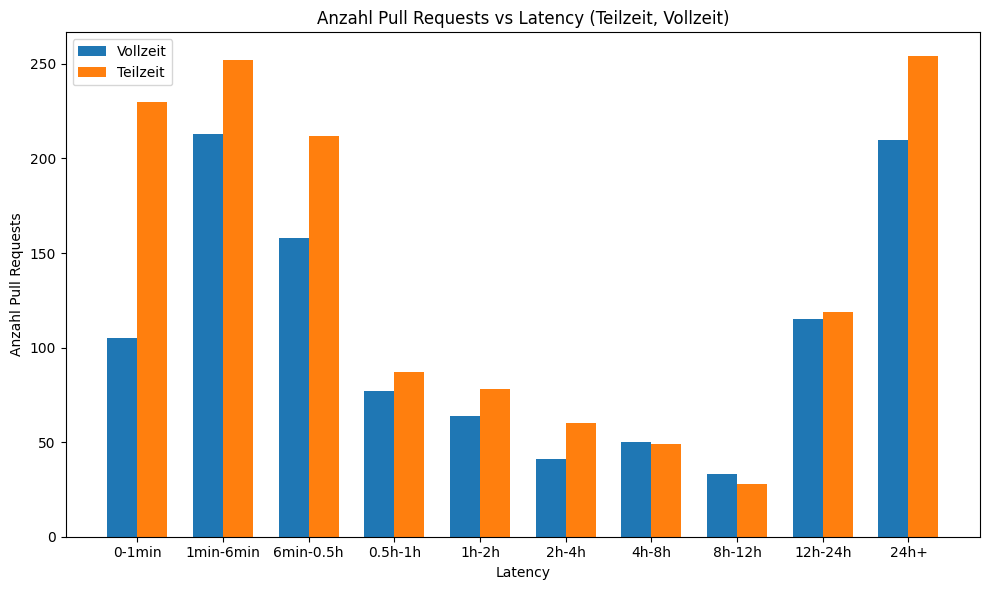
\includegraphics[width=\textwidth]{Figures/anz-prs-vs-latency-tv.png}
    \caption{Anzahl Pull Requests vs. Latency (Teilzeit, Vollzeit)}
    \label{fig:anz-prs-vs-latency-tv}
\end{figure}

Da in der Datenbasis mehr Teilzeitklassen und somit mehr Repositories vorhanden sind, werden die Daten auf die Anzahl der Repositories normiert, was eine unabhängigere Analyse ermöglicht.

Die \autoref{fig:anz-avg-prs-vs-latency-tv} zeigt nun, dass die Teilzeitstudierenden zwar immer noch viele Pull Requests innerhalb einer halben Stunde bearbeiten, aber nur im ersten Segment die Vollzeitstudierenden übertreffen. In den mittleren Intervallen sind die Teilzeitstudierenden relativ ausgeglichen, aber deutlich weniger als in den ersten drei Intervallen. Bei den Bearbeitungszeiten von mehr als sieben Tagen sind sie jedoch wieder stärker vertreten. Die Vollzeitstudierenden sind über alle Intervalle ausgeglichener, haben aber auch viele schnell bearbeiteten Pull Requests.


\begin{figure}[htbp]
    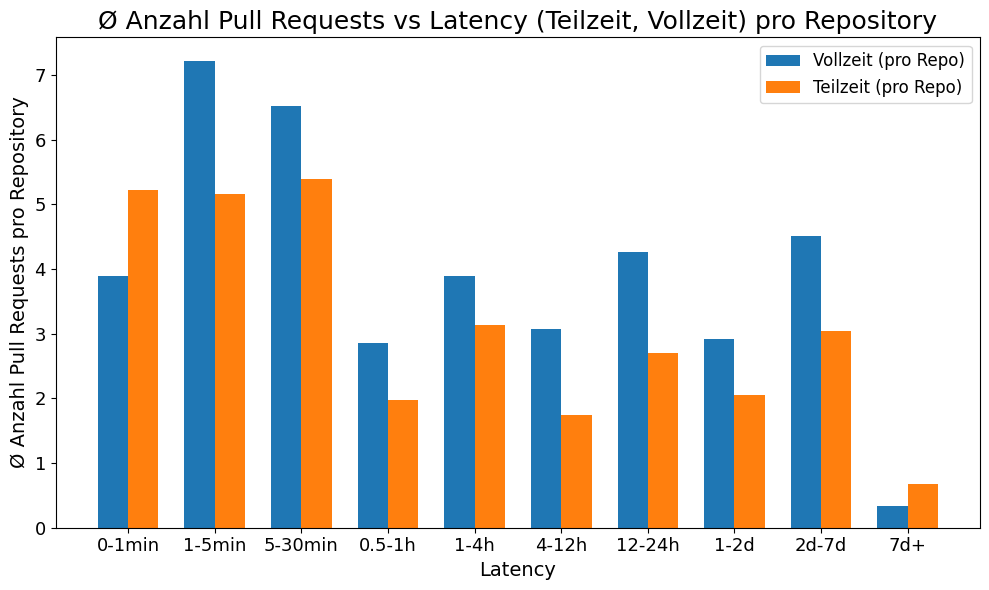
\includegraphics[width=\textwidth]{Figures/anz-avg-prs-vs-latency-tv.png}
    \caption{Durchschnittliche Anzahl Pull Requests vs. Latency (Teilzeit, Vollzeit)}
    \label{fig:anz-avg-prs-vs-latency-tv}
\end{figure}
\newpage
Insgesamt bestätigen die Abbildungen \autoref{fig:anz-prs-vs-latency-tv} und \autoref{fig:anz-avg-prs-vs-latency-tv}, dass die meisten Pull Requests schnell bearbeitet werden. Des Weiteren zeigt es, dass die Teilzeitstudierenden eine stärkere Streuung aufweisen als Vollzeitstudierende, da sie die Vollzeitstudierenden im ersten und letzten Intervall übertreffen.

// TODO Churn Latency
\newpage
Zur Klassifikation der Churn Grösse werden die von Doğan und Tüzün vorgeschlagenen Grössenkateogrien (XS, S, M, L, XL) verwendet. Diese Einteilung basiert auf empirischen Studien und industriellen Standards. \parencite{dogan_towards_2022}

Während der manuellen Untersuchung für die \fref{forschungsfrage2} wurde festgestellt, dass einige PRs einen Churn über 10'000 aufweisen. Entweder handelt es sich hierbei um geschlossene PRs welche entweder ausversehen erstellt oder beispielsweise mit dem falschen Zielbranch erstellt werden. Um diese zusätzlich klassifizieren zu können, wurde eine zusätzliche Grösse \textit{XXL} mit Churn \textit{10'000} erstellt. 

Somit ergibt sich für die Analyse folgende Klassifizierung: 
\begin{table}[ht]
\caption{Churn Grössenkategorien}
\label{tab:churnkategorien}
\centering
\begin{tabular}{l l}
\toprule
\textbf{Kategorie} & \textbf{Churn} \\
\midrule
XS  & 0--9       \\
S        & 10--49     \\
M        & 50--199    \\
L         & 200--999   \\
XL   & 1000--9999 \\
XXL  & 10000+ \\
\bottomrule
\end{tabular}
\end{table}


Abbildung \autoref{fig:anz-prs-vs-churn-size-tz-vz} zeigt die Pull Request der Voll- und Teilzeitklassen aufgeteilt nach ihrer Churn Grösse. So ist sichtbar, dass die Teilzeitklassen insegsamt mehr PRs erstellen. Dieser Trend ist in allen Grössenaktegorien sichtbar, ausser bei den \textit{XXL} PRs. Hier verfügen die Teilzeitklassen ingesamt über 2 PRs, während die Teilzeitklassen 5 PRs mit einem Churn über 10'000 verfügen. Bei den \textit{XXS} PRs verfügen die Teilzeitklassen über 1.5x so viele PRs.

\begin{figure}[htbp]
    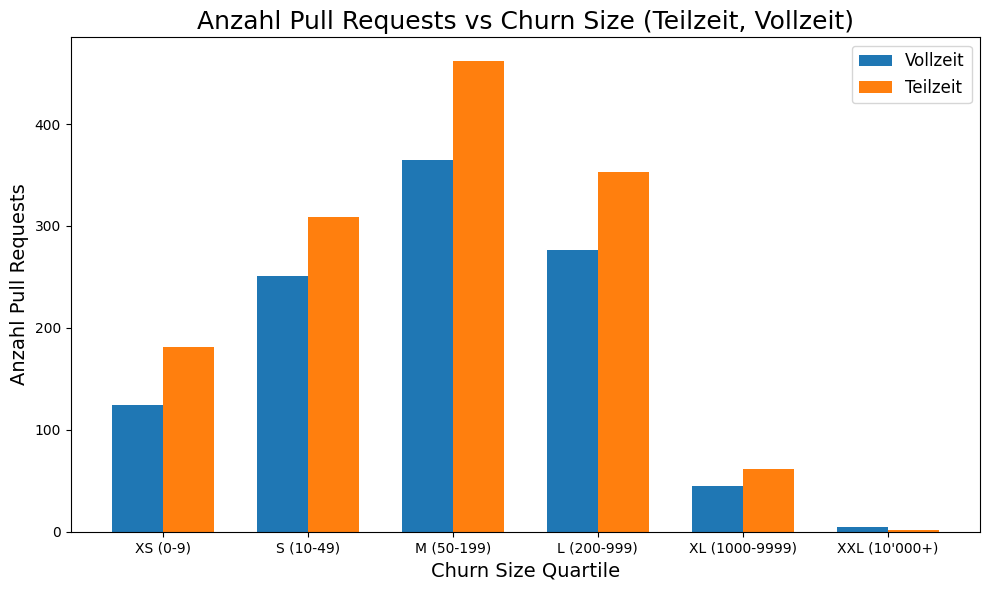
\includegraphics[width=\textwidth]{Figures/anz-prs-vs-churn-size-tz-vz.png}
    \caption{Anzahl PullRequests vs. Churn Grösse (Teilzeit, Vollzeit)}
    \label{fig:anz-prs-vs-churn-size-tz-vz}
\end{figure}

Eine Normalisierung der Daten pro Repo zeigt, dass die Vollzeitklassen entweder gleich viel oder mehr PRs pro Kategorie erstellen. Die Teilzeitklassen erstellen jedochh 

\begin{figure}[htbp]
    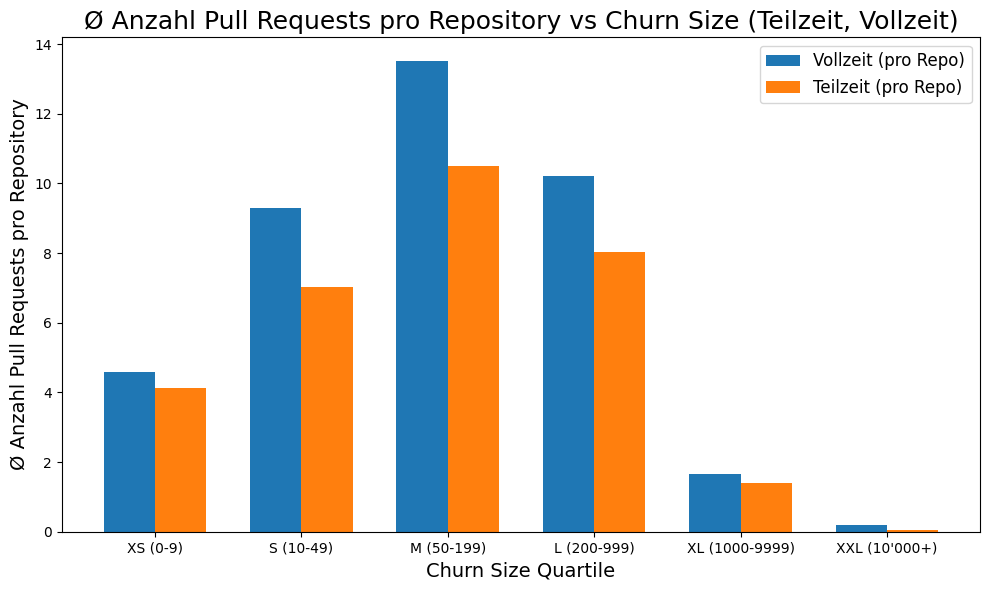
\includegraphics[width=\textwidth]{Figures/avg-anz-prs-vs-churn-size-tz-vz-pro-repo.png}
    \caption{Durchschnittliche Anzahl PullRequests vs. Churn Grösse pro Projekt(Teilzeit, Vollzeit)}
    \label{fig:anz-prs-vs-churn-size-tz-vz}
\end{figure}

Die für die \fref{forschungsfrage2} benötigte manuelle Untersuchung ergab, dass in einigen Klassen das in Kapitel \secref{sec:GitFlow} eingeführte Branching Konzept \textit{Git Flow} verwendet haben. Dies verfälscht eventuell die Daten, da es sich bei den manuell untersuchten Pull Requests um grosse PRs (Churn) handelt, welche keinen Review erfordern. Aus diesem Grund, werden die Analysen erneut durchgeführt jedoch mit herausgefilterten Dev Branches.

Da die Namen der Dev-Branches nicht einheitlich sind, werden alle Branches herausgefiltert, die das Wort Dev enthalten und auf den Main/Master Branch gemerged werden. Dabei ist zu beachten, dass GitHub den heutigen Haupt-Branch Main nennt, während dieser früher Master hiess. In der manuellen Analyse wurde festgestellt, dass einige Klassen aus dem Jahr 2021 immer noch solche Master Branches verwenden. Zusätzlich wurden alle herausgefilterten Pull Requests überprüft, um sicherzustellen, dass ausschliesslich Dev-Branches entfernt werden. Es wurden 75 Pull Requests von Dev-Branches zu Main-Branches ermittelt.


%// TODO anpassen wenn überhaupt beide grafiken
% Die Entfernung der Datensätze, welche Merges zwischen Developer-Branches und Main-Branches abbilden, verändert die Resultate marginal. Dies ist in der \autoref{fig:anz-prs-vs-latency-tv-no-dev} ersichtlich. Ebenso überwiegen in den ersten drei Spaltenpaaren und im letzten Paar die Teilzeitklassen. Am auffälligsten ist wiederum das erste Säulenpaar. Hier beträgt der Anteil der Teilzeitstudierenden an der Gesamtzahl der Teilzeitstudierenden 16 Prozent und bei den Vollzeitklassen 9.3 Prozent. Die Anzahl der Pull-Requests, die in weniger als einer Minute bearbeitet werden, ist also in beiden Klassen zurückgegangen, liegt aber in beiden Fällen unter einem Prozent.
% Addiert man die ersten drei Säulenpaare, so ergibt sich für die Teilzeitklassen ein Wert von 49.7 Prozent und für die Vollzeitklassen ein Wert von 43.3 Prozent. Damit liegen die Werte für die Teilzeit um genau ein Prozent und für die Vollzeit um 1.4 Prozent niedriger. Bei den 24 Stunden plus beträgt der Wert bei den Teilzeitklassen 19 Prozent, was einer Differenz von 0.4 Prozent entspricht. Bei den Vollzeitklassen beträgt der Wert 20.2 Prozent, was einem Anstieg von 0.5 Prozent gleichkommt.

% \begin{figure}[htbp]
%     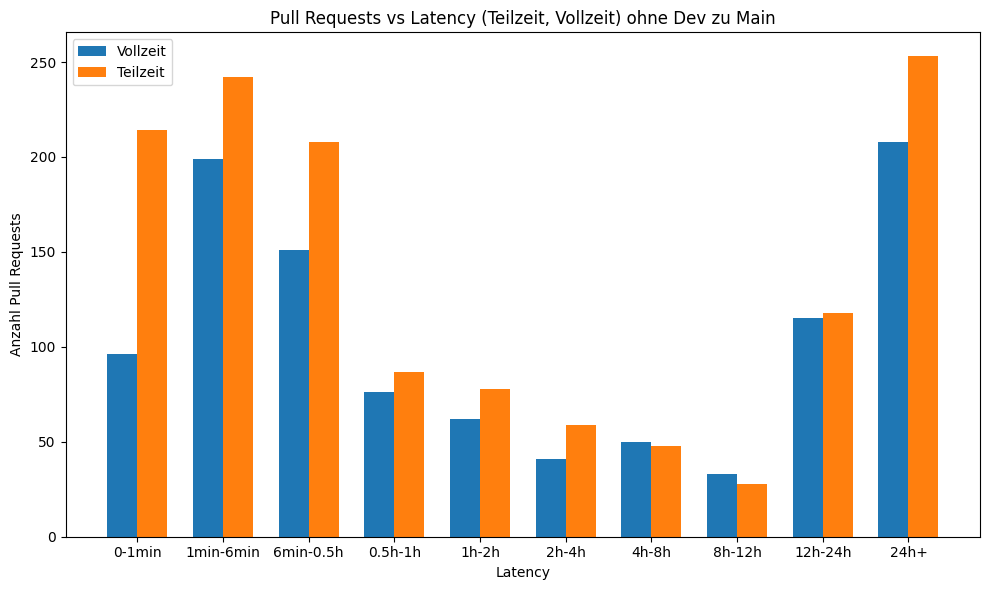
\includegraphics[width=\textwidth]{Figures/anz-prs-vs-latency-tv-no-dev.png}
%     \caption{Anzahl PullRequests vs. Latency (Teilzeit, Vollzeit) ohne Dev zu Main}
%     \label{fig:anz-prs-vs-latency-tv-no-dev}
% \end{figure}

Die \autoref{fig:anz-avg-prs-vs-latency-tv-no-dev} zeigt kaum Differenzen zur \autoref{fig:anz-avg-prs-vs-latency-tv}. Generell hat die durchschnittliche Anzahl der Pull Requests abgenommen, aber die Verteilung der Pull Requests unabhängig vom Unterrichtsmodell hat sich kaum verändert. 

\begin{figure}[htbp]
    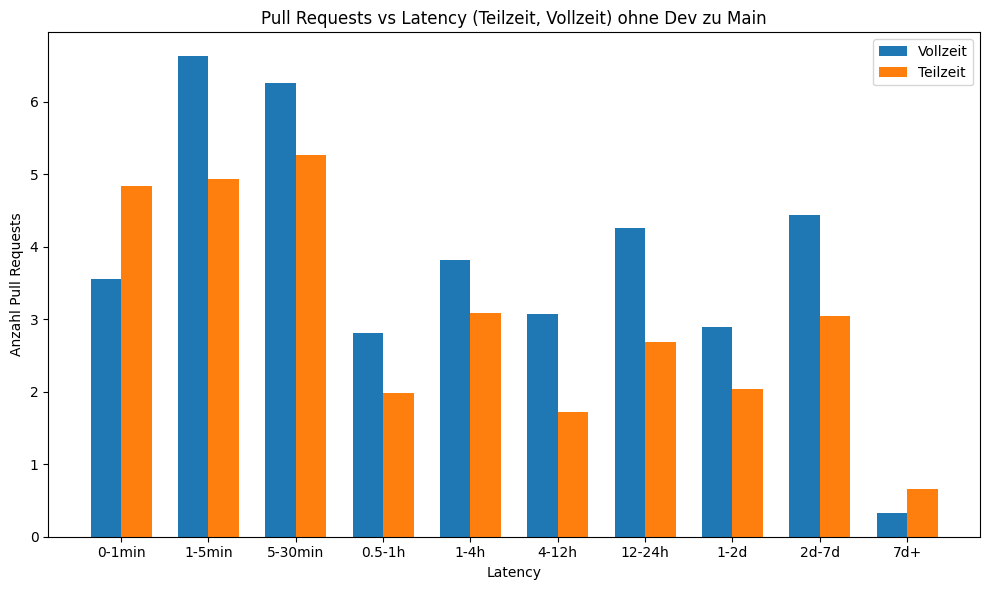
\includegraphics[width=\textwidth]{Figures/anz-avg-prs-vs-latency-tv-no-dev.png}
    \caption{Durchschnittliche Anzahl Pull Requests vs. Latency (Teilzeit, Vollzeit) ohne Dev zu Main}
    \label{fig:anz-avg-prs-vs-latency-tv-no-dev}
\end{figure}
\newpage

Somit zeigt sich, dass Dev-Branches keinen Einfluss auf die \textit{latencies} haben.



\subsection{Einfluss von Projektzeit}
Ein signifikanter Faktor, der bei Projektmodulen eine Rolle spielt, ist die fest definierte Abgabefrist. Dies unterscheidet diese Projekte von den Open-Source-Projekten, die in der Literatur häufig untersucht werden. Es soll nun untersucht werden, ob der Zeitpunkt der Erstellung eines Pull-Requests innerhalb der Projektlaufzeit einen Einfluss auf die Bearbeitung und vor allem auf die Dauer hat. Dafür wurde zusätzlich zu den oben genannten Metriken noch das Abgabedatum der einzelnen Klassen ermittelt. Da einige Dozenten ihr Feedback mittels Pull Request abgegeben haben, wurden alle Pull Requests herausgefiltert, die von einem Dozenten erstellt wurden. Dies wurde über das Attribut \textit{Author} ermittelt.

Es wurden verschiedene Analysen anhand eines Phyton Notebooks vorgenommen. Die erste Untersuchung analysierte, ob generell ein Zusammenhang über die \textit{latency} und \textit{churn} im Verlauf der Projektzeit festgestellt werden kann.  Um der in der Einleitung formulierten Hypothese nachzugehen, wurden die Pull Requests, die innerhalb von 30 Minuten und einer Minute gemerged wurden, ins Verhältnis zur Projektabgabe gesetzt und graphisch dargestellt. Des Weiteren wurden alle Pull Requests in Verbindung zur Abgabe gesetzt, um herauszufinden, wann die Pull Requests generell erstellt und bearbeitet wurden.  Darüber hinaus wurde analysiert, wie viele Pull Requests die Teams innerhalb der letzten 3 Projekttage und des letzten Projekttages noch abgearbeitet haben.
\subsection{Ergebnisse Einfluss Projektzeit}
Anhand der \autoref{fig:mittelwert-woche-lateny} ist ersichtlich, dass die Latency gegen Ende der Projektzeit abnimmt. Während die Churn (\autoref{fig:mittelwert-woche-churn}) bis zur 5. Woche ansteigt. 
Zu beachten ist, dass, wie bereits im Kapitel \secref{sec:Projektmodule} erwähnt, die Projekte nicht exakt 28 Tage dauern. Die ermittelten Projektlaufzeiten liegen zwischen 20 und 36 Tagen.
Wobei die Klassen aus den Jahren 2021 und 2022 bei einem Durchschnitt von 21 Tagen liegen. Die neueren Klassen ab dem Jahr 2023 haben eine Projektlaufzeitspannweite von 28 bis 36 Tagen. Wovon eine Klasse die 35 Tage überschreitet. In dieser Klasse haben fünf Teams eine Laufzeit von 29 Tagen und drei Teams eine Laufzeit von 35 oder 36 Tagen. Somit widerspiegeln diese drei Teams die Woche sechs in der folgenden \autoref{fig:vergleich-latency-churn-projektzeit}. Die Latency nimmt im Laufe der Zeit zweimal stark ab. Das erste Mal von der ersten zur zweiten Projektwoche, wobei sie in der ersten Woche bei einem Mittelwert von 3.5 Stunden und in der zweiten Woche bei 2 Stunden liegt. Zum zweiten Mal nimmt die Latenz in der vierten Projektwoche stark ab, und zwar von 1.7 Stunden auf 0.5 Stunden. In der sechsten Woche ist die Latency nahezu 0. Der Churn steigt bis zur 5. Woche kontinuierlich von 72 Zeilenwechseln auf 115 an und sinkt dann in der 6. Woche auf 98.
\begin{figure}[htbp]
    \centering
    \begin{subfigure}[b]{0.48\textwidth}
        \centering
        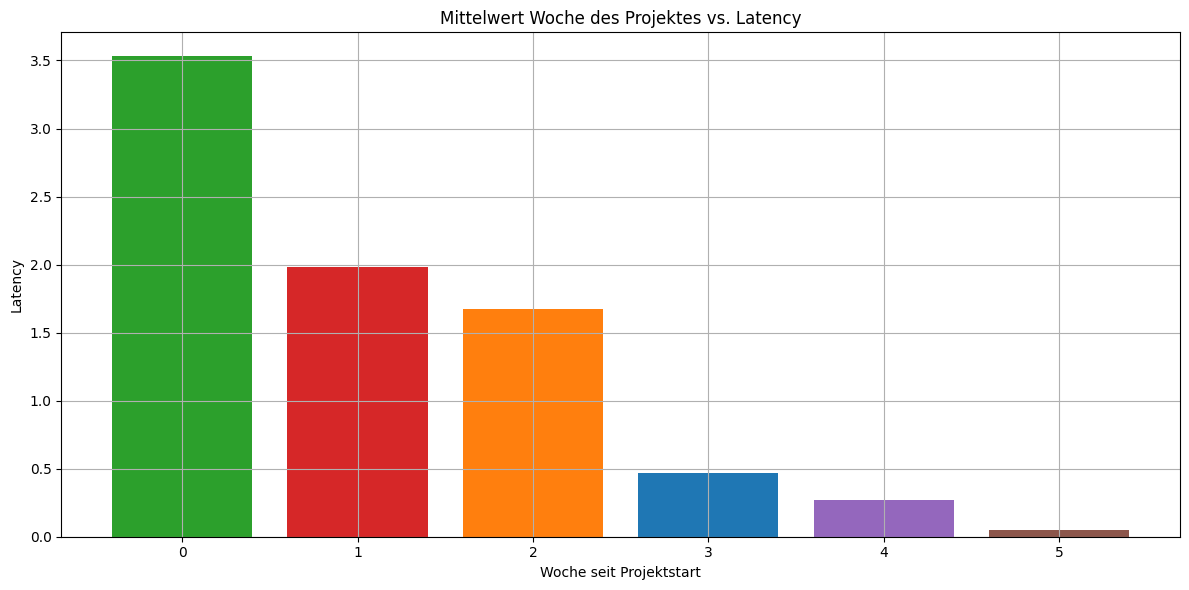
\includegraphics[width=\textwidth]{Figures/mittelwert-woche-lateny.png}
        \caption{Mittelwerte Woche des Projektes vs. Latency}
        \label{fig:mittelwert-woche-lateny}
    \end{subfigure}
    \hfill
    \begin{subfigure}[b]{0.48\textwidth}
        \centering
        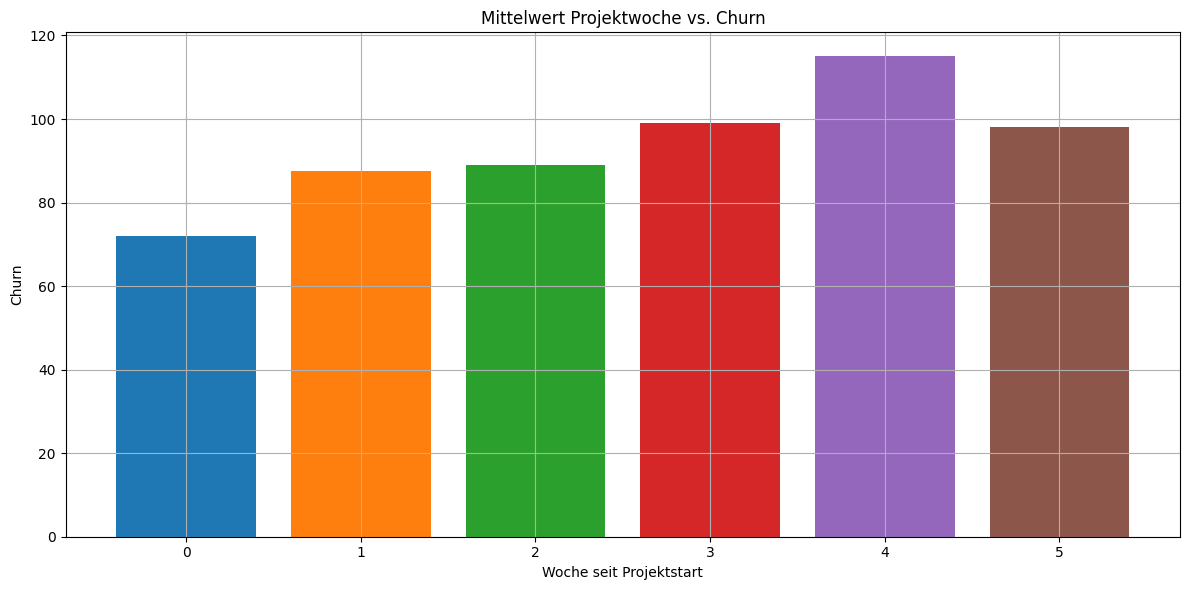
\includegraphics[width=\textwidth]{Figures/mittelwert-woche-churn.png}
        \caption{Mittelwerte Woche des Projektes vs. Churn}
        \label{fig:mittelwert-woche-churn}
    \end{subfigure}
    \caption{Vergleich von Latency und Churn innerhalb der Projektzeit}
    \label{fig:vergleich-latency-churn-projektzeit}
\end{figure}

Werden die Daten nach Vollzeit- und Teilzeitstudierenden aufgeteilt, zeigt sich bei den Vollzeitklassen ein ähnliches Bild. Veranschaulicht wird dies in der \autoref{fig:vergleich-latency-churn-projektzeit-v}. Allerdings ist der Mittelwert der Latecy in der ersten Woche mit 7.4 Stunden mehr als doppelt so hoch wie in der Gesamtauswertung. Ebenso nimmt die Latency von der ersten zur zweiten Woche stark ab. Der Wert sinkt um mehr als die Hälfte und liegt anschliessend bei 3.4 Stunden. Ab der vierten Woche ist der Mittelwert unter einer halben Stunde. Zeitgleich ist der Churn in der ersten Woche mit 71 Zeilenänderungen am geringsten, steigt mit Ausnahme der dritten Woche an und erreicht in der fünften Woche mit 121 Änderungen seinen Höhepunkt. Im Gegensatz zur Latency liegen diese Werte sehr nahe bei der Gesamtanalyse.
\begin{figure}[htbp]
    \centering
    \begin{subfigure}[b]{0.48\textwidth}
        \centering
        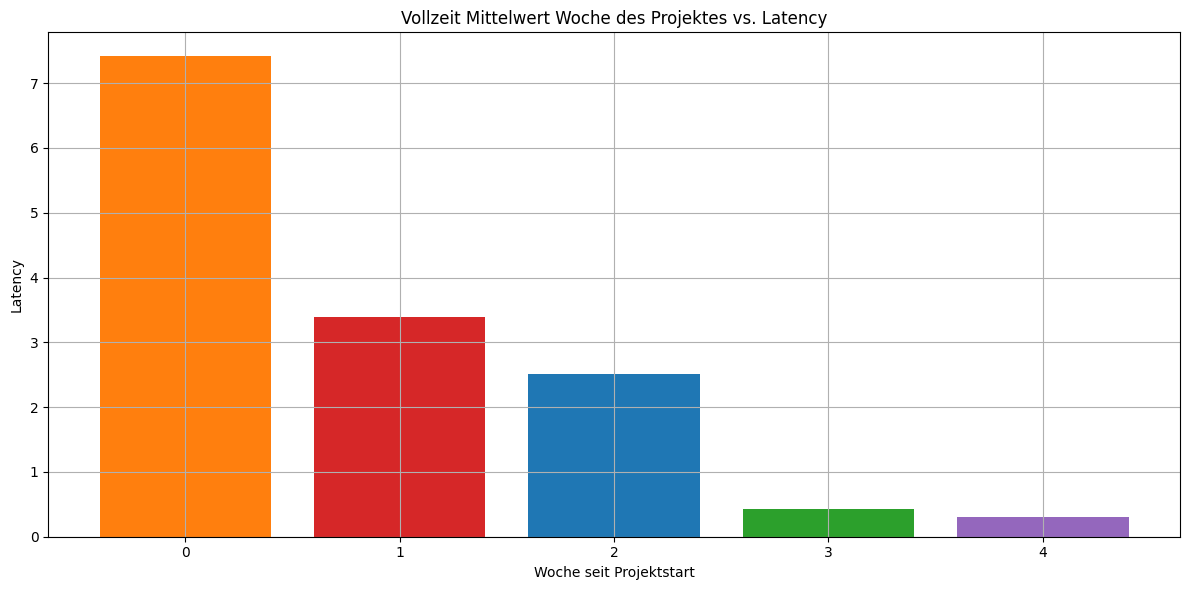
\includegraphics[width=\textwidth]{Figures/mittelwert-woche-lateny-v.png}
        \caption{Mittelwerte Woche des Projektes vs. Latency Vollzeit}
        \label{fig:mittelwert-woche-lateny-v}
    \end{subfigure}
    \hfill
    \begin{subfigure}[b]{0.48\textwidth}
        \centering
        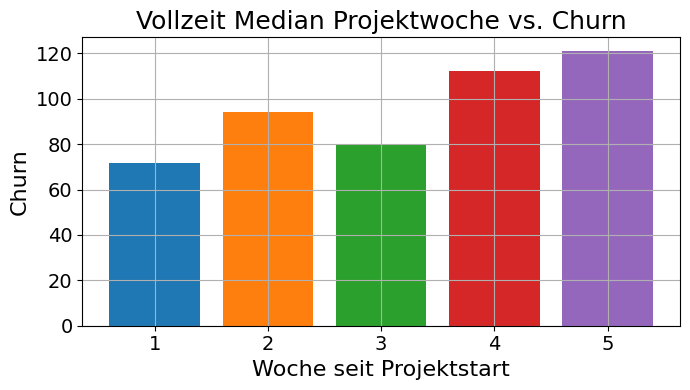
\includegraphics[width=\textwidth]{Figures/mittelwert-woche-churn-v.png}
        \caption{Mittelwerte Woche des Projektes vs. Churn Vollzeit}
        \label{fig:mittelwert-woche-churn-v}
    \end{subfigure}
    \caption{Vergleich von Latency und Churn innerhalb der Projektzeit Vollzeit}
    \label{fig:vergleich-latency-churn-projektzeit-v}
\end{figure}

In der \autoref{fig:vergleich-latency-churn-projektzeit-t} ist zu erkennen, dass auch bei den Teilzeitstudierenden die Latency in der ersten Woche am höchsten ist, sich aber weniger stark von den Wochen zwei und drei unterscheidet. Zusätzlich ist der Wert der ersten Woche im Gegensatz zur Gesamtanalyse und vor allem den Vollzeitstudierenden tiefer bei einem Wert von knapp 2 Stunden. Zudem steigt bei den Teilzeitklassen in der dritten Woche die Latency nochmals an, aber dies nur mit einem Unterschied von 0.1 Stunden. Danach sinkt die Latency ebenso und liegt in Woche vier unter einer Stunde. Der Churn steigt ebenfalls an und erreicht in Woche fünf seinen Höhepunkt bei 110 Codezeilenänderungen. Die Werte der Churn befinden sich im gleichen Rahmen wie bei den Vollzeitstudierenden.

\begin{figure}[htbp]
    \centering
    \begin{subfigure}[b]{0.48\textwidth}
        \centering
        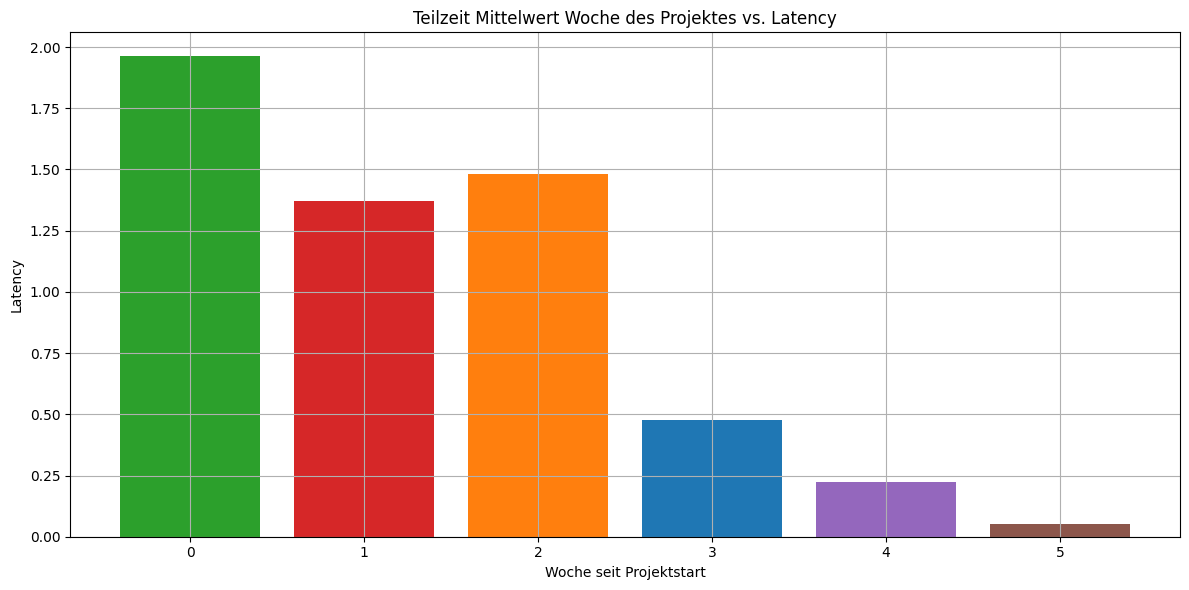
\includegraphics[width=\textwidth]{Figures/mittelwert-woche-lateny-t.png}
        \caption{Mittelwerte Woche des Projektes vs. Latency Teilzeit}
        \label{fig:mittelwert-woche-lateny-t}
    \end{subfigure}
    \hfill
    \begin{subfigure}[b]{0.48\textwidth}
        \centering
        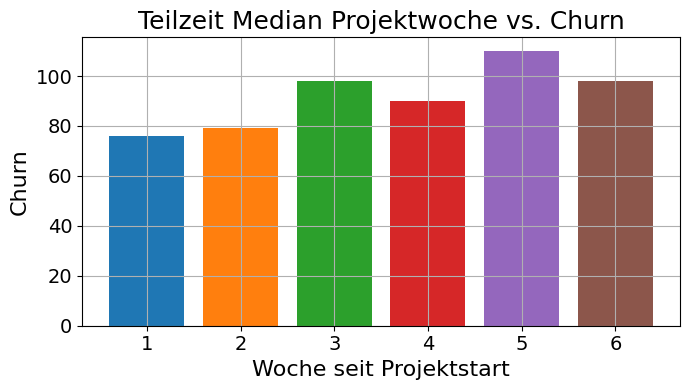
\includegraphics[width=\textwidth]{Figures/mittelwert-woche-churn-t.png}
        \caption{Mittelwerte Woche des Projektes vs. Churn Teilzeit}
        \label{fig:mittelwert-woche-churn-t}
    \end{subfigure}
    \caption{Vergleich von Latency und Churn innerhalb der Projektzeit Teilzeit}
    \label{fig:vergleich-latency-churn-projektzeit-t}
\end{figure}

\newpage
Die Analyse der Daten, die in der \autoref{fig:anz-prs-vs-latency-tv} dargestellt sind, zeigt, dass eine Vielzahl von PullRequests innerhalb einer halben Stunde bearbeitet wurde. Eine detaillierte Analyse dieser kurz geöffneten PullRequests offenbart, dass der überwiegende Teil davon in den letzten drei Tagen und insbesondere am Tag der Abgabe erstellt wurde. Eine weitere Restriktion der Pull Requests auf jene, die innerhalb einer Minute abgearbeitet wurden, resultiert in einer ähnlichen Situation. Es ist jedoch festzustellen, dass der Tag der Abgabe sich stärker abhebt, wobei auch ein Anstieg zwei Tage vor Abgabe zu erkennen ist.  Die Resultate sind in \autoref{fig:anz-prs-under-x-mins} dargestellt.

\begin{figure}[htbp]
    \centering
    \begin{subfigure}[b]{0.48\textwidth}
        \centering
        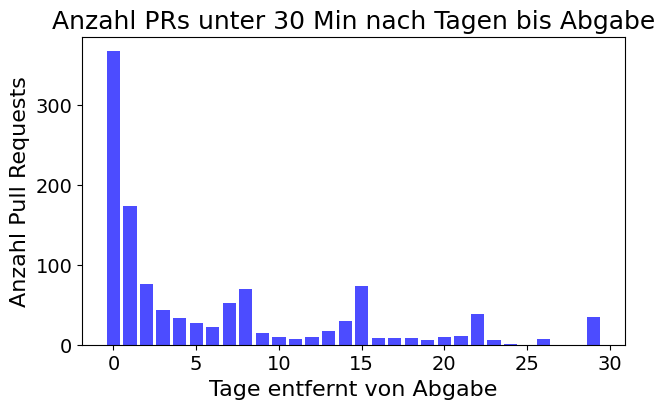
\includegraphics[width=\textwidth]{Figures/anz-prs-under-30-min.png}
    \caption{Anzahl PullRequests unter 30 Minuten im Verhältnis zur Abgabe}
    \label{fig:anz-prs-under-30-min}
    \end{subfigure}
    \hfill
    \begin{subfigure}[b]{0.48\textwidth}
        \centering
        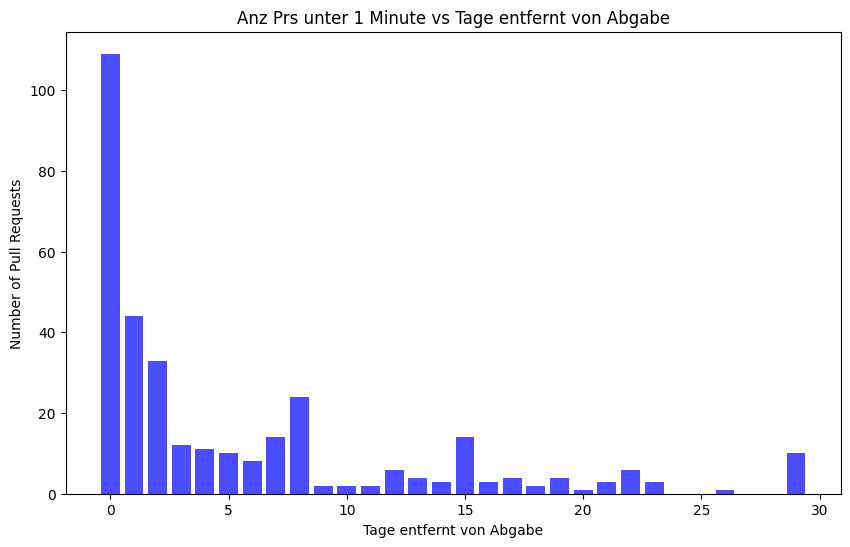
\includegraphics[width=\textwidth]{Figures/anz-prs-under-1-min.png}
    \caption{Anzahl PullRequests unter einer Minute im Verhältnis zur Abgabe}
    \label{fig:anz-prs-under-1-min}
    \end{subfigure}
    \caption{Anzahl PullRequests unter 30 / 1 Minute im Verhältnis zur Abgabe}
    \label{fig:anz-prs-under-x-mins}
\end{figure}

Die Untersuchung von Pull Requests im Verhältnis zur Abgabe zeigt, dass am Tag der Abgabe die meisten Pull Requests abgearbeitet wurden. Dies ist aus der \autoref{fig:anz-prs-days-away-from-end} ersichtlich. Von den 2427 untersuchten Pull Requests wurden 523 am Tag der Abgabe erstellt und abgeschlossen. Dieser Wert entspricht einer Quote von 21.5 Prozent.  Die zweitmeisten Pull Request wurden am Tag vor der Abgabe bearbeitet mit einer Anzahl von 309. Am drittletzten Tag wurde ein erhöhter Wert festgestellt, der jedoch nicht mehr signifikant hervorsticht. Es wurden 154 Pull Requests bearbeitet. Eine Zusammenfassung der letzten drei Tage der Projekte ergibt eine Gesamtzahl von 986 bearbeiteten Pull Requests, was einem Prozentsatz von 40.6 Prozent entspricht. Über die restliche Projektzeit variieren die Anzahl bearbeiteten Pull Rquests. Es lassen sich erhöhte Werte sieben, acht und 15 Tage vor der Abgabe feststellen, die sich von den Werten der übrigen Tage abheben.
\begin{figure}[htbp]
    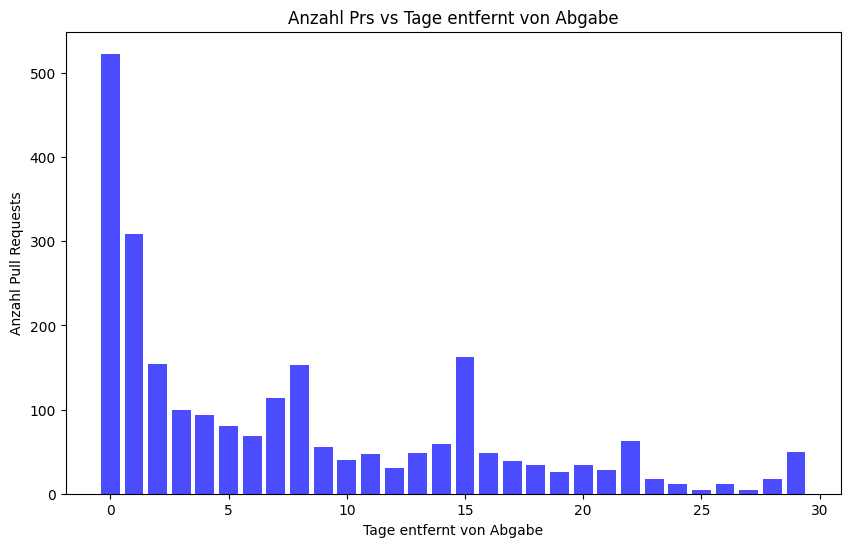
\includegraphics[width=\textwidth]{Figures/anz-prs-days-away-from-end.png}
    \caption{Anzahl geschlossene Pull Requests im Verhältnis zur Abgabe}
    \label{fig:anz-prs-days-away-from-end}
\end{figure}
\newpage
Eine detaillierte Analyse der Pull Requests in den einzelnen Teams zeigt, dass in 19 von 71 Teams mehr als 50 Prozent aller Pull Requests in den letzten drei Projekttagen eröffnet und abgeschlossen wurden. Es lässt sich feststellen, dass vier der analysierten Teams einen Anteil von über 75 Prozent ihrer Pull Requests in diesem Zeitraum bearbeitet haben. Zudem ist eine Gruppe zu identifizieren, die sämtliche ihrer Pull Requests innerhalb des definierten Zeitraums erstellt und geschlossen hat. Eine detaillierte Analyse des Projektes ergab, dass die genannte Gruppe insgesamt zwei Pull Requests hatte, die beide am Tag vor der Abgabe erstellt wurden. Wenn diese Analyse auf den letzten Projekttag beschränkt wird, dann sind es drei Teams, die mehr als 50 Prozent ihrer Pull Requests am Abgabetag erledigt haben.

\section{Ergebnisse Pull Reqeust Akzeptanz}
Die aktuelle Literatur zeigt, dass sowohl soziale und prozessbezogene Faktoren als auch technische Merkmale berücksichtigt werden müssen. 

Um die Ursache des geschlossenen PRs zu gruppieren, wurden folgende Gruppen erstellt: 
\begin{itemize}
    \item \textbf{PRs ohne erkennbaren Grund}: Die PRs wurden ohne Kommentar geschlossen. Die Churn Grösse ist kleiner als 500. 
    \item \textbf{Issue / Feature durch anderen PR implementiert}: Das Feature wurde durch einen anderen PR implementiert und anschliessend dann geschlossen. 
    \item \textbf{PRs mit falschem Zielbranch}: Der Autor des PRs wählte den falschen Zielbranch aus. Der PR wurde anschliessend in einen anderen Branch gemerdet. 
    \item \textbf{Feature wird nicht mehr benötigt}: Das Feature wird nicht mehr benötigt. Diess muss so im PR vermerkt sein. 
    \item \textbf{Implementierung abgelehnt}: Die Implementierung wurde abgelehnt. 
\end{itemize}


Für die Analyse der geschlossenen Pull Requests (PRs) wurden zunächst alle verfügbaren PRs eingelesen und entsprechend gefiltert. Erste Auswertungen ergaben, dass lediglich 0,07\% aller Pull Requests geschlossen wurden. Von den insgesamt 170 geschlossenen PRs entfallen 95 auf die Vollzeitklassen und 75 auf die Teilzeitklassen, obwohl der analysierte Datenbestand 27 Vollzeitprojekte und 43 Teilzeitprojekte umfasst. Der durchschnittliche Churn der PRs liegt in den Teilzeitklassen ebenfalls niedriger (137 im Vergleich zu 188 bei den Vollzeitklassen).

Abbildung \autoref{fig:anz-clsd-prs-nach-churn} zeigt die Anzahl geschlossener PRs, gruppiert nach ihrer Churn-Grösse. Dabei wird deutlich, dass in den Teilzeitklassen vor allem kleinere PRs abgelehnt wurden. Eine manuelle Analyse der Gründe für das Scheitern dieser PRs ergab, dass viele ohne jeglichen Kommentar abgelehnt wurden. Ob dies daran lag, dass die Implementierung nicht mehr benötigt wurde oder fehlerhaft war, lässt sich im Nachhinein nicht eindeutig klären.

\begin{figure}[htbp]
    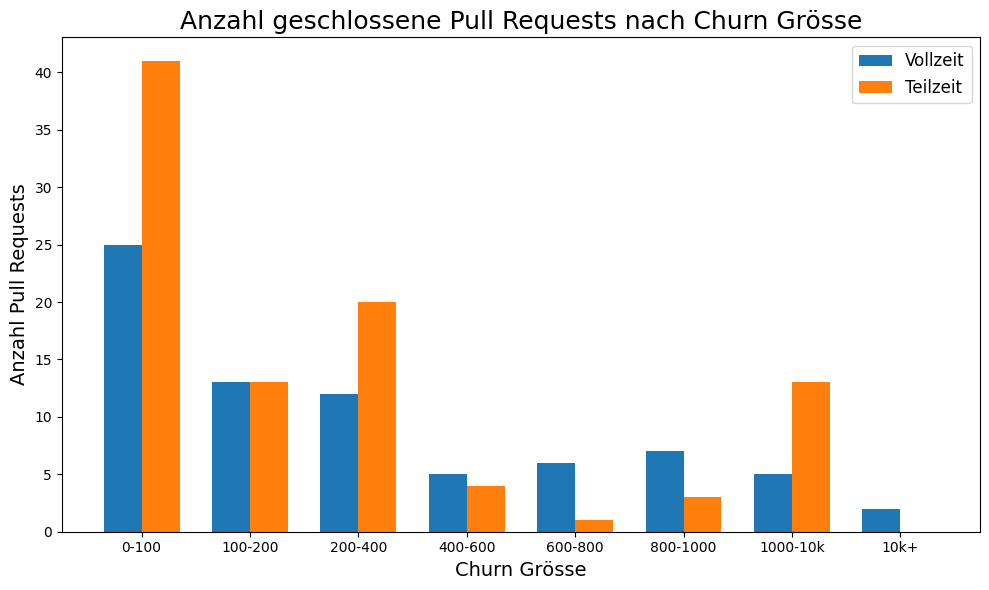
\includegraphics[width=\textwidth]{Figures/anzahl-geschlossene-prs-nach-churn.png}
    \caption{Anzahl geschlossene Pull Requests nach Churn Grösse}
    \label{fig:anz-clsd-prs-nach-churn}
\end{figure}


Die manuelle Analyse der geschlossenen PRs mit einem Churn von über 500 zeigte hingegen ein anderes Bild: Diese PRs wurden häufig aufgrund eines falschen Zielbranches erstellt. In mehreren Fällen konnte ausserdem beobachtet werden, dass das vorgeschlagene Feature bereits durch einen anderen Branch implementiert worden war. Gewisse PRs wurden auch für grosse Refactoring Arbeiten verwendet. 

Die Kategorie 'divers' beinhaltet hauptsächlich Feedback-PRs, welche von gewissen Dozenten für die Notenvergabe verwendet wurden. Ausserdem sind einige refactor Branches zu sehen, welche Ausschliesslich für den Refactoren erstellt wurden und anschliessend geschlossen wurden. 

\begin{table}
\caption{Geschlossene PRs gruppiert nach Ursache}
\label{tab:treatments}
\centering
\begin{tabular}{l l l l l l l}
\toprule
\textbf{Klasse} & 
\makecell{\textbf{PR abgelehnt} \\ \textbf{ohne Grund}} & 
\makecell{\textbf{Feat. durch} \\ \textbf{anderen PR impl.}} & 
\makecell{\textbf{Feat. nicht} \\ \textbf{mehr benötigt}} & 
\makecell{\textbf{Impl.} \\ \textbf{abgelehnt}} & 
\makecell{\textbf{falscher} \\ \textbf{Zielbranch}} &
\makecell{\textbf{divers}} \\
\midrule
T < 100& 35 & 1 & 3 & 2 & 0 & 0\\
V < 100& 22 & 1 & 0 & 1 & 1 & 0 \\
T > 500& 22 & 8 & 0 & 2 & 4 & 5 \\
V > 500& 8 & 0 & 1 & 4 & 6 & 0 \\
\bottomrule
\end{tabular}
\end{table}
\newpage
\noindent\textbf{Legende:}
\begin{itemize}
\item[$T$] Alle Teilzeitklassen
\item[$V$] Alle Vollzeitklassen
\item[$< 100$] Churn kleiner 100
\item[$> 500$] Churn grösser 500
\end{itemize}

\subsection{Ergebnisse Einfluss Projektzeit}
Wie in Abbildung \autoref{fig:closed-prs-projektkeit-teilzeit} deutlich wird, wurden die meisten Pull Requests (PRs) in den Teilzeitklassen am letzten Tag vor der Projektabgabe geschlossen. Dieser Effekt ist zwar auch in den Vollzeitklassen erkennbar, jedoch weniger ausgeprägt. In Abbildung \autoref{fig:closed-prs-projektkeit-vollzeit} wird zudem deutlich, dass die geschlossenen PRs in den Vollzeitklassen gleichmässiger über den gesamten Projektzeitraum verteilt sind.

\begin{figure}[htbp]
    \centering
    \begin{subfigure}[b]{0.48\textwidth}
        \centering
        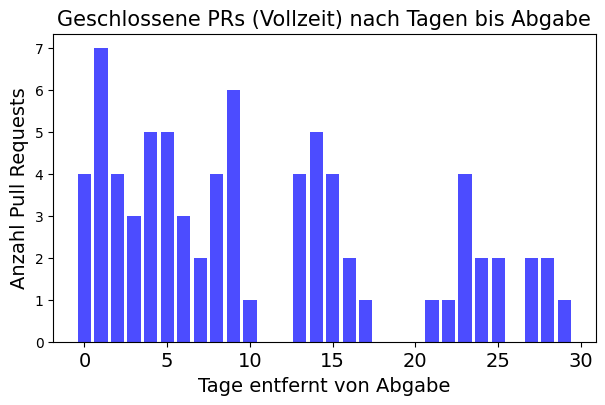
\includegraphics[width=\textwidth]{Figures/closed-prs-projektzeit-vollzeit.png}
        \caption{Anzahl geschlossene PRs Vollzeitklassen nach Tagen entfernt von Abgabe}
        \label{fig:closed-prs-projektkeit-vollzeit}
    \end{subfigure}
    \hfill
    \begin{subfigure}[b]{0.48\textwidth}
        \centering
        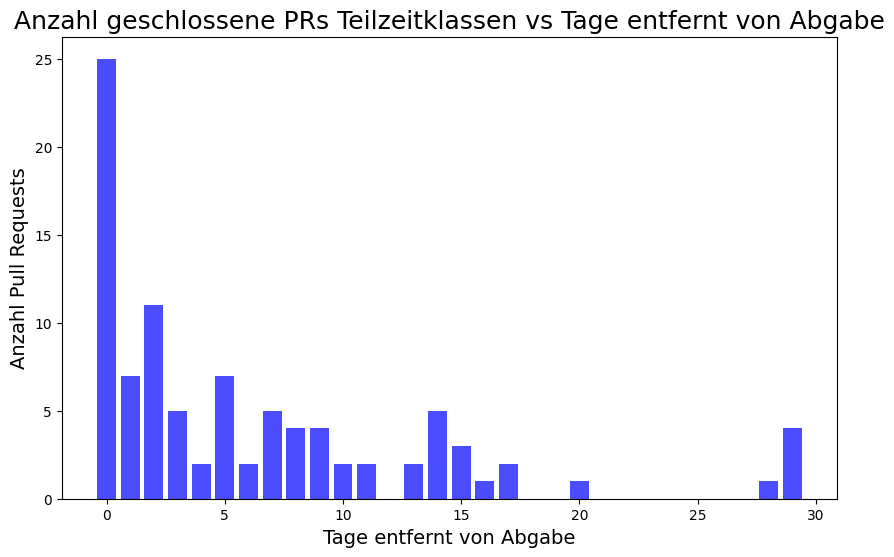
\includegraphics[width=\textwidth]{Figures/closed-prs-projektzeit-teilzeit.png}
         \caption{Anzahl geschlossene PRs Teilzeitklassen nach Tagen entfernt von Abgabe}
        \label{fig:closed-prs-projektkeit-teilzeit}
    \end{subfigure}
    \caption{Vergleich Anzahl geschlossene PRs Teilzeit vs Vollzeit nach Tagen entfernt von Abgabe}
    \label{fig:vergleich-latency-churn-projektzeit}
\end{figure}


\section{Ergebnisse Entwicklungsaktivität}
Für die Analyse der Entwicklungsaktivität wurde das Jupyter Notebook \textit{analyse-wochen-latency-churn.ipynb} erstellt \parencite{stumpf_simon_repo-detectivesba-metric-analysis-scripts_nodate}. 

Um die Entwicklungsaktivität messbar machen zu können, mussten für alle Klassen die Projektmodul-Unterrichtstage ermittelt werden:
\begin{table}[ht]
\caption{Projektmodul-Unterrichtstage der Klassen}
\label{tab:stundenplan}
\centering
\begin{tabular}{l l l}
\toprule
\textbf{Klasse} & \textbf{Ort} & \textbf{Tag} \\
\midrule
It21tb   & Zürich      & Montag      \\
It21ta   & Zürich      & Montag      \\
It21a    & Zürich      & Mittwoch    \\
It21tb   & Winterthur  & Donnerstag  \\
It21a    & Winterthur  & Freitag     \\
It21b    & Winterthur  & Freitag     \\
It21ta   & Winterthur  & Freitag     \\
\midrule
It23tb   & Zürich      & Montag      \\
It23ta   & Zürich      & Montag      \\
It23a    & Zürich      & Mittwoch    \\
It23b    & Zürich      & Mittwoch    \\
It23a    & Winterthur  & Freitag     \\
It23ta   & Winterthur  & Freitag     \\
It23tb   & Winterthur  & Freitag     \\
\midrule
It24tb   & Zürich      & Montag      \\
It24ta   & Zürich      & Montag      \\
It24a    & Zürich      & Mittwoch    \\
It24a    & Winterthur  & Freitag     \\
It24ta   & Winterthur  & Freitag     \\
It24tb   & Winterthur  & Freitag     \\
\bottomrule
\end{tabular}
\end{table}

Empirische Studien zeigen, dass die Entwicklungsaktivität in Open-Source-Projekten auf Plattformen wie GitHub charakteristische Muster im Wochenverlauf aufweist. Insbesondere an Wochenenden ist die Aktivität signifikant geringer als unter der Woche. Innerhalb der Arbeitswoche fallen Montag und Freitag häufig als die Tage mit der geringsten Aktivität auf. Das Phänomen des Rückgangs der Entwicklungsaktivität wird oftmals auch \textit{Friday Effect} genannt. \parencite{claes_programmers_2018}

Da sich während der Analyse deutliche Differenzen zwischen den Voll- und Teilzeitklassen ergaben, wurden diese in der Analyse geteilt angeschaut. 

Auch in den vorliegenden Daten zeigt sich eine Tendenz zur Konzentration der Aktivitäten auf spezifische Wochentage, insbesondere auf die jeweiligen Unterrichtstage. So wurden bei den Vollzeitklassen rund 24\,\% aller Pull Requests (PRs) am Projekttag erstellt. Bei den Teilzeitklassen liegt dieser Wert mit 34\,\% deutlich höher. Dies unterstreicht die Bedeutung des Unterrichtstages für die praktische Arbeit im Rahmen des Projekts.

Abbildung \autoref{fig:anz-prs-teilzeit-pro-wochentag} zeigt exemplarisch die Verteilung der PR-Erstellungen über die Wochentage für zwei Teilzeitklassen. Deutlich erkennbar ist ein Aktivitätspeak am jeweiligen Unterrichtstag. An den darauffolgenden Tagen nimmt die Aktivität deutlich ab. Auffällig ist zudem, dass PRs nicht nur am Unterrichtstag erstellt, sondern auch überprüft und geschlossen wurden. Insgesamt wurden 27.7\,\% aller PRs der Teilzeitklassen am Wochenende erstellt – ein vergleichsweise hoher Wert.

\begin{figure}[htbp]
    \centering
    \begin{subfigure}[b]{0.48\textwidth}
        \centering
        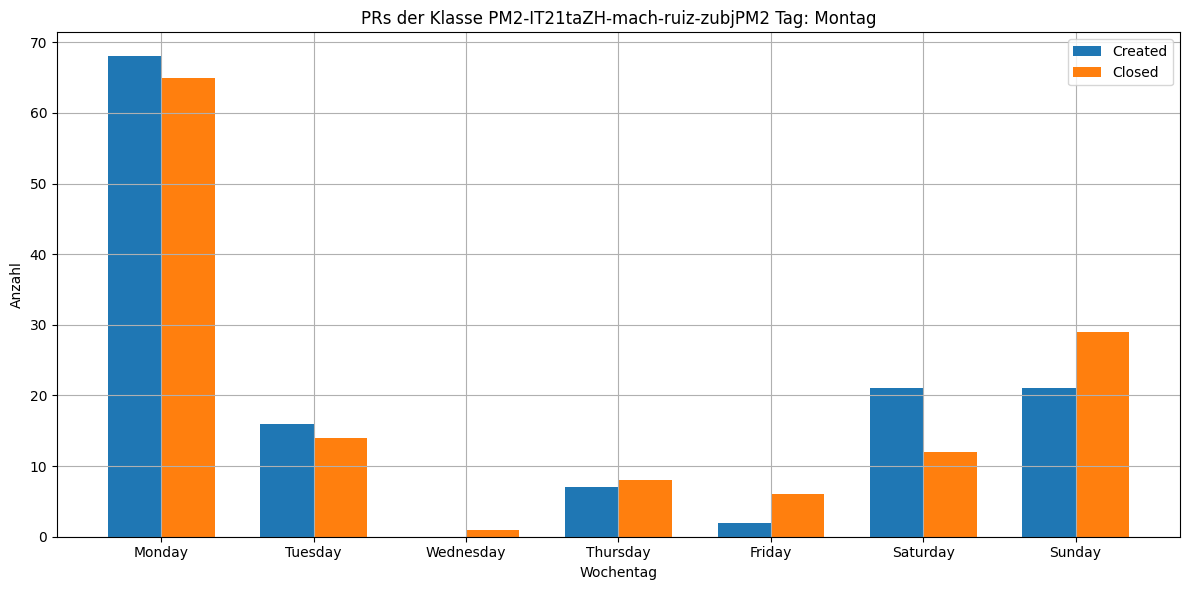
\includegraphics[width=\textwidth]{Figures/pr-klasse-per-wochentag-it21ta.png}
         \caption{Anzahl geöffneter PRs pro Wochentag der Teilzeitklasse It21ta}
        \label{fig:anzahl-prs-pro-wochentag-it21ta}
    \end{subfigure}
    \hfill
    \begin{subfigure}[b]{0.48\textwidth}
        \centering
        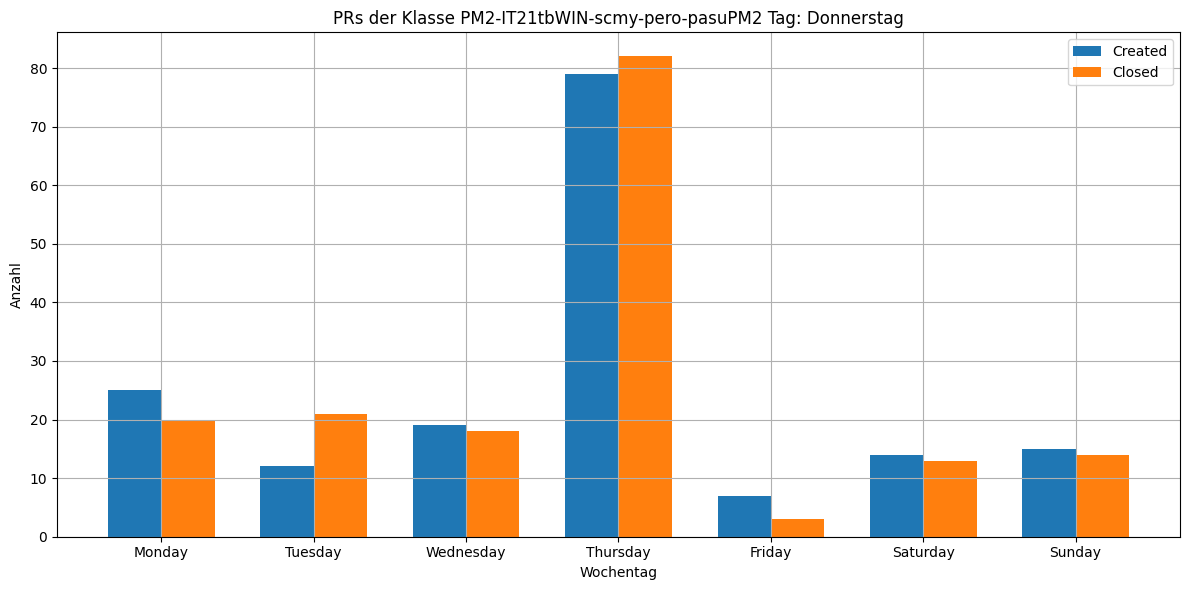
\includegraphics[width=\textwidth]{Figures/pr-klasse-per-wochentag-21tb.png}
         \caption{Anzahl geöffneter PRs pro Wochentag der Teilzeitklasse It21tb}
        \label{fig:anzahl-prs-pro-wochentag-it21tb}
    \end{subfigure}
    \caption{Anzahl geöffneter PRs pro Wochentag von 2 Teilzeitklassen}
    \label{fig:anz-prs-teilzeit-pro-wochentag}
\end{figure}

Ein kontrastierendes Bild zeigt sich bei den Vollzeitklassen. Abbildung \autoref{fig:anz-prs-vollzeit-pro-wochentag} zeigt die Verteilung der PR-Erstellungen bei zwei exemplarischen Klassen. 
Hier zeigt sich eine insgesamt gleichmässigere Verteilung der Aktivitäten über die Woche. Zwar ist auch hier der Projekttag der aktivste, jedoch in geringerem Ausmass als bei den Teilzeitklassen. Zudem wurden nur 16.8\% der PRs am Wochenende erstellt.

\begin{figure}[htbp]
    \centering
    \begin{subfigure}[b]{0.48\textwidth}
        \centering
        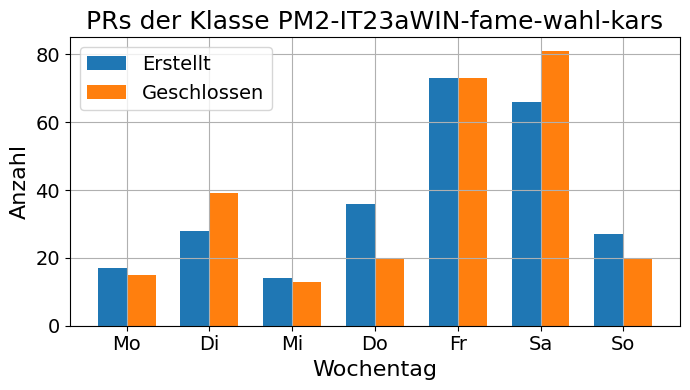
\includegraphics[width=\textwidth]{Figures/pr-klasse-per-wochentag-23a.png}
         \caption{Anzahl geöffneter PRs pro Wochentag der Vollzeitklasse It23a}
        \label{fig:anzahl-prs-pro-wochentag-it23a}
    \end{subfigure}
    \hfill
    \begin{subfigure}[b]{0.48\textwidth}
        \centering
        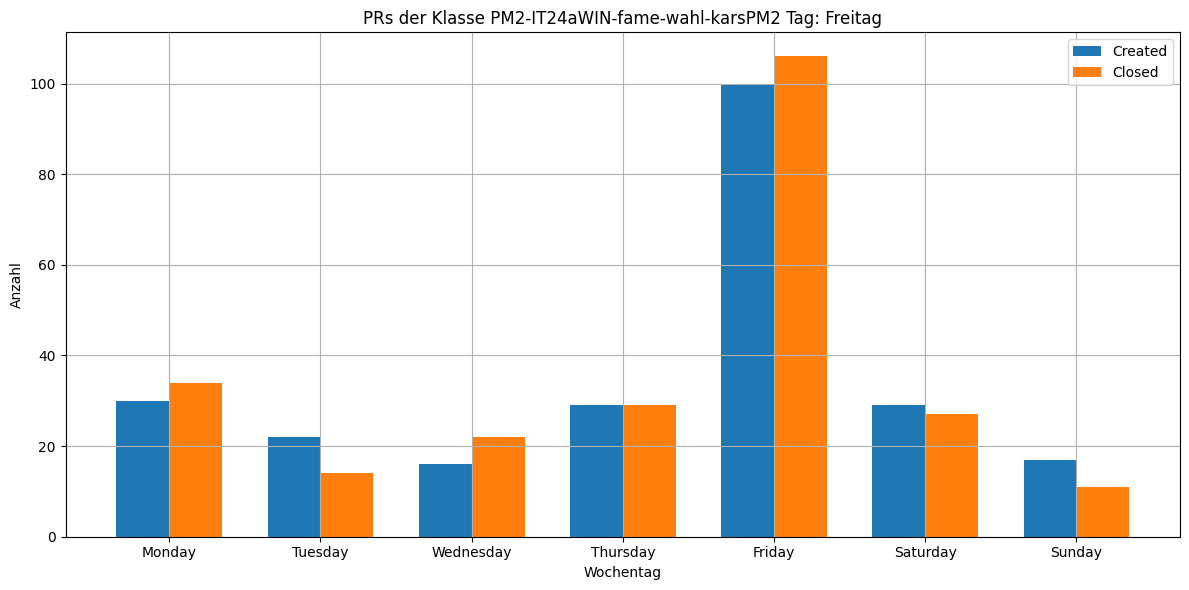
\includegraphics[width=\textwidth]{Figures/pr-klasse-per-wochentag-24a.png}
         \caption{Anzahl geöffneter PRs pro Wochentag der Vollzeitklasse It24a}
        \label{fig:anzahl-prs-pro-wochentag-it24a}
    \end{subfigure}
    \caption{Anzahl geöffneter PRs pro Wochentag von 2 Vollzeitklassen}
    \label{fig:anz-prs-vollzeit-pro-wochentag}
\end{figure}

\subsection{Ereignisse Analyse Commits}
Da nicht nur die PRs sondern auch die einzelnen Commits interessant für die Entwicklungsanalyse ist, wurden die Commits der PRs angeschaut. 
Die Analyse bestätigte die Resultate, welche in der PR Analyse bereits schon gefunden wurden. 

So wurden bei den Vollzeitklassen 23.7\,\% aller Commits am jeweiligen Unterrichtstag durchgeführt. Bei den Teilzeitklassen liegt dieser Anteil mit 33.9\,\% deutlich höher. Abbildung \autoref{fig:anz-commits-teilzeit-pro-wochentag} zeigt die Verteilung der Commits über die Wochentage exemplarisch für zwei Teilzeitklassen. Erkennbar ist – analog zur PR-Verteilung – ein deutlicher Peak an den jeweiligen Projekttagen. Insgesamt wurden 25.9\,\% aller Commits der Teilzeitklassen an einem Samstag oder Sonntag durchgeführt.

\begin{figure}[htbp]
    \centering
    \begin{subfigure}[b]{0.48\textwidth}
        \centering
        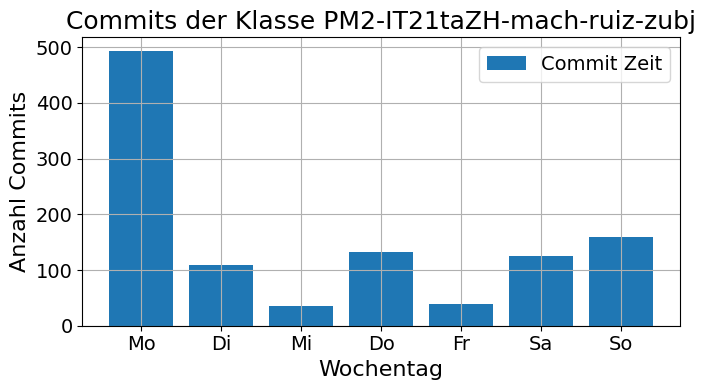
\includegraphics[width=\textwidth]{Figures/commits-klasse-per-wochentag-21ta.png}
         \caption{Anzahl Commits pro Wochentag der Teilzeitklasse It21ta}
        \label{fig:anzahl-commits-pro-wochentag-it21ta}
    \end{subfigure}
    \hfill
    \begin{subfigure}[b]{0.48\textwidth}
        \centering
        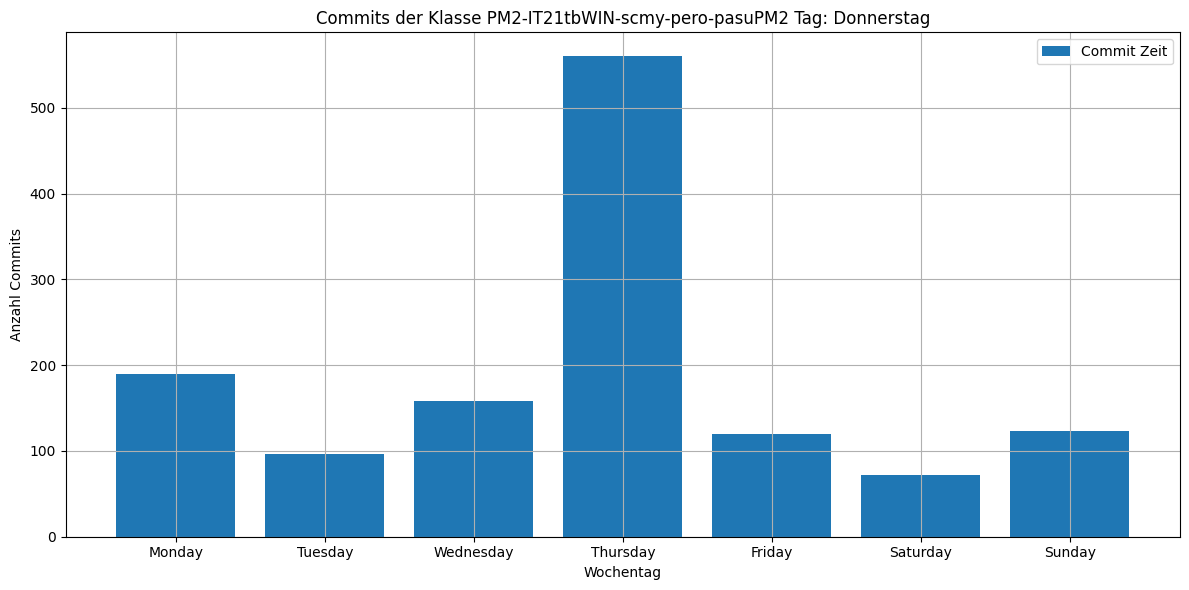
\includegraphics[width=\textwidth]{Figures/commits-klasse-per-wochentag-21tb.png}
         \caption{Anzahl Commits pro Wochentag der Teilzeitklasse It21tb}
        \label{fig:anzahl-commits-pro-wochentag-it21tb}
    \end{subfigure}
    \caption{Anzahl Commits pro Wochentag von 2 Teilzeitklassen}
    \label{fig:anz-commits-teilzeit-pro-wochentag}
\end{figure}

Ein ähnliches Bild ergibt sich bei den Vollzeitklassen. Abbildung \autoref{fig:anz-commits-vollzeit-pro-wochentag} zeigt die Commits zweier exemplarischer Klassen. Hier wurden 23.7\,\% der Commits am jeweiligen Projekttag durchgeführt – identisch mit dem PR-Anteil. Am Wochenende hingegen wurden nur 19.4\,\% der Commits verzeichnet, was deutlich unter dem Wert der Teilzeitklassen liegt.

\begin{figure}[htbp]
    \centering
    \begin{subfigure}[b]{0.48\textwidth}
        \centering
        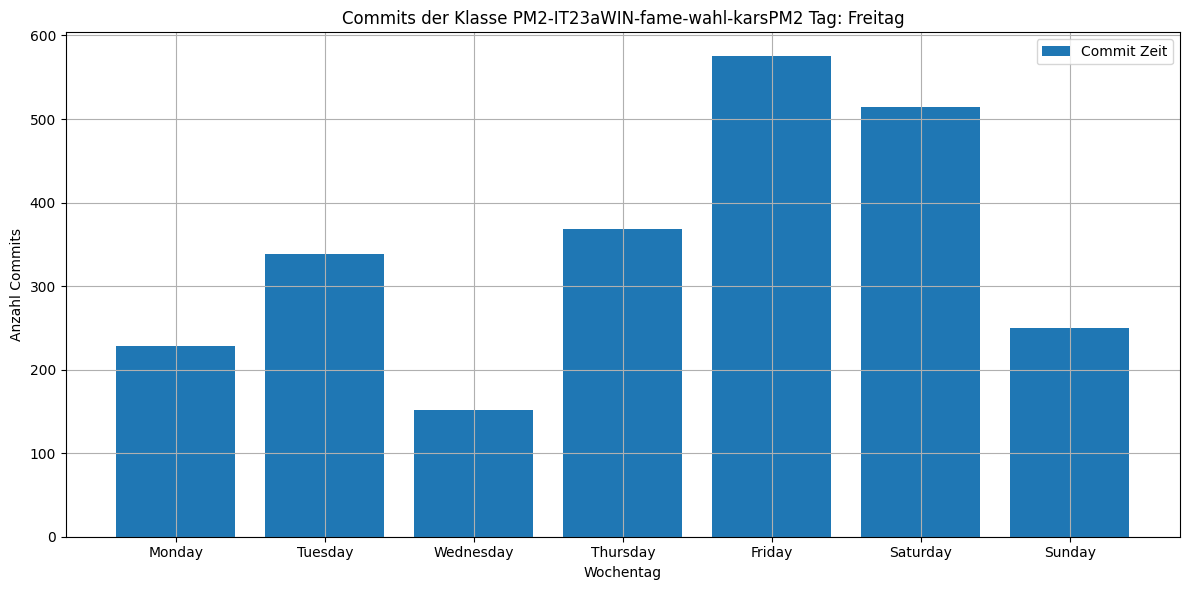
\includegraphics[width=\textwidth]{Figures/commits-klasse-per-wochentag-23a.png}
         \caption{Anzahl Commits pro Wochentag der Teilzeitklasse It23a}
        \label{fig:anzahl-commits-pro-wochentag-it23a}
    \end{subfigure}
    \hfill
    \begin{subfigure}[b]{0.48\textwidth}
        \centering
        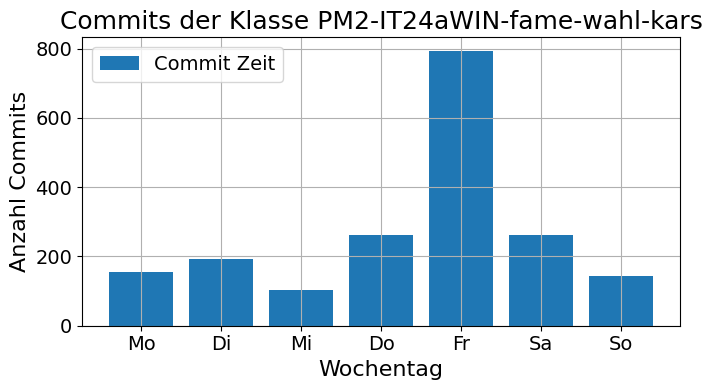
\includegraphics[width=\textwidth]{Figures/commits-klasse-per-wochentag-24a.png}
         \caption{Anzahl Commits pro Wochentag der Teilzeitklasse It24a}
        \label{fig:anzahl-commits-pro-wochentag-it24a}
    \end{subfigure}
    \caption{Anzahl Commits pro Wochentag von 2 Vollzeitklassen}
    \label{fig:anz-commits-vollzeit-pro-wochentag}
\end{figure}

\section{Projektmodul Ergebnisse bei Open Source Projekten}
\subsection{Latency und Churn}
\subsection{Allgemeine Korrelationen}

